
\chapter{Metaphoricity Of Compositions With Distributional Representations}
\chaptersource{Yuri Bizzoni, Stergios Chatzikyriakidis and Mehdi Ghanimifard.}{``Deep'' Learning: Detecting Metaphoricity in Adjective-Noun Pairs.}{In Proceedings of the Workshop on Stylistic Variation, pp. 43-52. 2017.}


\paragraph{Abstract}
Metaphor is one of the most studied and widespread figures of speech and an essential element of individual style. In this paper we look at metaphor identification in Adjective-Noun pairs. We show that using a single neural network combined with pre-trained vector embeddings can outperform the state of the art in terms of accuracy. In specific, the approach presented in this paper is based on two ideas: a) transfer learning via using pre-trained vectors representing adjective noun pairs, and b) a neural network as a model of composition that predicts a metaphoricity score as output. We present several different architectures for our system and evaluate their performances. Variations on dataset size and on the kinds of embeddings are also investigated.  We show considerable improvement over the previous approaches both in terms of accuracy and w.r.t the size of annotated training data.


\section{Introduction}



The importance of metaphor to characterize both individual and genre-related style has been underlined in several works \citep{leech2007style,simpson2004stylistics,goodman1975status}. Studying the kinds of metaphors used in a text can contribute to differentiate between poetic and prosaic style, etc. In literary studies, metaphor analysis is often undertaken on a stylistic perspective: "after all, metaphor in literature is a stylistic device and its forms, meanings and use all fall within the remit of stylistics" \cite{steen2014metaphor}. Metaphor is thus often taken into consideration  qualitative stylistic analyses \citep{fahnestock2009quid}. Nonetheless, it is still very difficult to take metaphors into account in computational stylistics due to the complexity of automatic metaphor identification \citep{neuman2013metaphor,klebanov2015supervised}, which is the task of identifying metaphorical usages of text, sentences or subsentential fragments. 


This paper's focus of interest is the automatic detection of adjective-noun (AN) pairs like the following:
\begin{itemize}[topsep=0em,itemsep=0em,partopsep=0em,parsep=0em]
	\item Clean floor / clean performance
	\item Bright painting / bright idea
	\item Heavy table / heavy feeling
\end{itemize}
The above examples illustrate that adjectives  ``normally" used to describe physical characteristics, e.g. a feature that can be perceived through senses like size or weight, are reused to describe more abstract properties. Thus, both a painting and an idea can be bright, both a table and a feeling can be heavy. We will not provide a mean to retrieve AN metaphors in unconstrained texts (e.g. we won't focus on segmentation) but we will study ways to detect metaphoricity in given pairs. Theoretical work on metaphor in the linguistics literature goes back a long way and spans different theoretical paradigms. One of the earliest and most influential works is Conceptual Metaphor Theory (CMT) \cite{Lakoff:2008} (originally published in 1981) and subsequently elaborated in a couple of papers \cite{lakoff1989some,lakoff1993contemporary}. According to CMT, metaphors in natural language can be seen as instances of conceptual metaphors. A conceptual metaphor  roughly corresponds to understanding a concept or an idea via association or relation with another idea or concept. Other influential linguistic approaches to metaphor include pragmatic approaches cast within frameworks like relevance theory \cite{romero2014relevance,wilson2011parallels},  and also approaches where some sort of formal semantics is used   \cite{vogel2001dynamic}. The common denominator in all these approaches  is the recognition that there is systematicity in the way metaphorical meanings arise and also that the process of metaphor construction is extremely productive. Thus, given these properties, one would expect metaphors to be quite common in Natural Language (NL). Evidence from corpus linguistics  seems to support this claim \cite{cameron2003metaphor}. 

Metaphor detection in statistical NLP has been attempted through several different frames, such as topic modeling \cite{Li:2010:UGM:1857999.1858038}, semantic similarity graphs \citep{li:2010}, distributional clustering \citep{shutova:2010}, vector space based learning \cite{gutierrez2016literal} and, most of all, feature-based classifiers \cite{Tsvetkov_metaphordetection}. In the latter case, the challenge consists in selecting the right features to annotate the training data with, and to review their "importance" or weight based on machine learning results. 

In this paper we show how using a single-layered neural network combined with pre-trained distributional embeddings can outperform the state of the art in an AN metaphor detection task. 

More specifically, this paper's contributions are the following:
\begin{itemize}[topsep=0em,itemsep=0em,partopsep=0em,parsep=0em]
\item We introduce a system to predict AN metaphoricity and test  it on the corpus introduced by \cite{gutierrez2016literal}, showing a significant improvement in accuracy.
\item We explore different variations of this model based on ideas found in the literature for composing distributional meaning and we evaluate them under different constraints. 
\end{itemize}
The paper is structured as follows: in Section 2 we present the background on AN metaphor detection and we detail the dataset we use to train our model. 
In Section 3 we describe our approach, giving a general overview and further describing three alternative architectures on the same model. 
In Section 4 we present several evaluations of our model. Table~\ref{others:table} and Table~\ref{stylevar2017:tab:arch} synthesize some of our findings. 
In Section 5 we discuss our findings and possible future applications of the work described in this paper. 

\begin{table*}
	\begin{center}
	\begin{tabular}{| l | c | c | c | c |}
	 \hline 
	 & \rotatebox{90}{Accuracy} & \rotatebox{90}{Feature engineering} &  \rotatebox{90}{Annotated dataset} & \rotatebox{90}{Embedding} \\
	 \hline 
	\cite{Turney:2011:LMS:2145432.2145511} & 0.79 & Yes  & 100 & LSA\\ \hline 
	\cite{Tsvetkov_metaphordetection} & 0.85 & Yes  & 200 & - \\ \hline 
	\cite{gutierrez2016literal} & 0.81 & No  & 8592 & DSM\\ \hline 
	Our model & \textbf{0.91} & No  & 8592 & Word2Vec\\ \hline 
	\end{tabular}
	\vspace{0.5em}
	\caption{\label{others:table} The reported accuracy from previous words on AN metaphor detection. The first two studies used different datasets. We are using larger pre-trained vectors than \citet{gutierrez2016literal}; at the same time, we don't need a parsed corpus to build our vectors and we don't use adjectival matrices. Given these differences, this comparison should not be considered a ``competition".}
	\end{center}
\end{table*}

\begin{table}[t]
	\centering
	\begin{tabular}{|l|r|r|}
	\hline
	{} &  \textbf{Random} $W$ &   \textbf{Trained} $W$ \\
	\hline
	cat-linear &  0.8973 &  0.9153 \\\hline
	cat-relu   &  0.8763 &  0.9228 \\\hline
	sum-linear &  0.8815 &  0.9068 \\\hline
	sum-relu   &  0.8597 &  0.9150 \\\hline
	mul-linear &  0.7858 &  0.8066 \\\hline
	mul-relu   &  0.7795 &  0.8186 \\\hline
	\end{tabular}
	\vspace{0.5em}
	\caption{\label{stylevar2017:tab:arch} The accuracy results after training the model based on each architecture. In all setups, we trained on 500 samples in 20 epochs. Using a random W is equivalent to preventing our network from learning any form of compositionality (we could consider it as a baseline for models with trained W). As we discuss in the paper, the difference in accuracies with the ``baseline" (not training W) shows that training W is helpful. }
\end{table}


\section{Background}

In the specific task of detecting metaphoricity for AN pairs we find four relevant works that seem to represent the main stages in figurative language detection until now. 

The oldest work of the series, \cite{Krishnakumaran:2007:HEM:1611528.1611531}, strongly relies on external resources. They adopt a WordNet based approach to recognize Noun-Noun (NN), Noun-Verb (NV) and AN metaphors.  Their work is mainly based on qualitative analyses of specific examples and shows that, while they can be useful in such a task, hyponym/hypernym relations  are not enough to distinguish metaphors from literal expressions. 

More recently, \citet{Turney:2011:LMS:2145432.2145511} adopt a two-stage machine learning approach. They first try to learn the words' degree of concreteness and then use this knowledge to detect whether an AN couple is metaphorical or not. They measure their performance on 100 phrases involving 5 adjectives and reach an accuracy of 0.79. It is worth noting that this choice is not random: the authors select the abstract/concrete polarity based on psycholinguistic findings that seem to validate the hypothesis that some kinds of metaphorical expressions are  processed as abstract elements.\footnote{For a more recent study on this issue see \cite{cogni15}.}

These results were outperformed by \citet{Tsvetkov_metaphordetection} through a random forest classifier using DSM vectors, WordNet senses and several accurately selected features, such as abstractness. They also introduce a new set of 200 phrases, on which they declare an F-score of 0.85.

Finally, \citet{gutierrez2016literal} train a distributional model on a corpus of 4.58 billion tokens and test it on an annotated dataset they introduce consisting of 8592 AN phrases. This is the same dataset we are using in this paper and the largest available to date. 

They first train distributional vectors for the words in the dataset using positive pointwise mutual information.
Then, for each adjective present in the dataset, they divide the literal phrases the adjective occurs in from the metaphorical phrases the same adjective appears in.   Then, three different adjective matrices are trained: one to model the adjective's literal sense, one to model its metaphorical sense, and one trained on all the phrases containing this adjective, both literal and metaphorical. They then develop a system to ``decide" whether a particular occurrence of an adjective is more likely to relate to the ``literal matrix" or the ``metaphorical matrix". It is shown that, although such matrices are trained on relatively few examples, they can reach an accuracy of over 0.78.  


\subsection{Corpus/Experimental Data}


The dataset we are using comes from \cite{gutierrez2016literal}. \footnote{The dataset is publicly available here:  http://bit.ly/1TQ5czN} It contains 8592 annotated
AN pairs, 3991 being literal and 4601 being metaphorical. The dataset focuses on a set of 23 adjectives that: a) can potentially have both metaphorical and literal meanings, and b) are fairly productive.

The choice of adjectives was based on the test set of \cite{Tsvetkov_metaphordetection} and focuses on 23 adjectives.

In details, all adjectives belong to one of the following categories: 
\begin{enumerate}[topsep=0em,itemsep=0em,partopsep=0em,parsep=0em]
\item  temperature adjectives (e.g. cold)
\item  light adjectives (e.g. bright)
\item  texture adjectives (e.g. rough)
\item  substance adjectives (e.g. dense)
\item  clarity adjectives (e.g. clean)
\item  taste adjectives (e.g. bitter)
\item  strength adjectives (e.g. strong)
\item   depth adjectives (e.g. deep)
\end{enumerate}

The corpus was carefully built in order to avoid non-ambiguous elements: all the AN phrases present in this dataset were extracted from large corpora and all phrases that seemed to require a larger context for their interpretation were filtered out in order to eliminate potentially ambiguous idiomatic expressions such as \textit{bright side}. 

In other terms, the corpus was designed to contain elements whose metaphoricity could be deduced by a human annotator without the need of a larger context. 

More details about the construction of the dataset and annotation 
methodology can be found in \cite{gutierrez2016literal}.

\section{Describing our approach}

\subsection{The model framework}

Our objective is to build a classifier that disambiguates between metaphoric and literal AN compositions by providing a probability measure between 0 and 1. We based the framework of the model on the following ideas:
\begin{enumerate}[topsep=0em,itemsep=0em,partopsep=0em,parsep=0em]
	\item Transfer learning: we use pre-trained word-vectors to represent AN pairs as input. 
	\item A neural network as a model of composition for the AN phrase: our model represents phrases with vectors, then based on this representation predicts a metaphoricity score as output. Although we are going to present several variations of this framework, it's important to remember that the basic model is always a standard NN with a single fully connected hidden layer we will call \textbf{p}.
\end{enumerate}
Our approach is thus based on the idea that well-trained distributional vectors contain more valuable information than their reciprocal similarity and, furthermore, that it is possible to treasure such information through machine learning in different tasks. We use 300-dimensional word vectors trained on different corpora (see Evaluation for more details) . Our approach can be considered as a way of transferring the learned representation from one task to another. Although it is not possible to point out an explicit mapping between the word-vector learning task (e.g. Word2Vec model) and our metaphoricity task, as it is pointed out by \citealt{torrey2009transfer}, we use neural networks which automatically learn how to adapt the feature representations between two tasks \cite{bengio2013representation}.  In this way we stretch the original embeddings, trained in order to learn lexical similarity, to identify AN metaphors.

Our neural network, being a parameterized function, follows the generalized architecture of word-vector composition similar to \cite{mitchell2010composition}:
\begin{equation}\label{eq:composition}
\mathbf{p} = f(\mathbf{u}, \mathbf{v}; \theta)
\end{equation}
where $\mathbf{u}$ and $\mathbf{v}$ are two word vector representations to be composed, while $\mathbf{p}$ is the vector representation of their composition with the same dimensions. The function $f$ in our model is parameterized by $\theta$, a list of parameters to be learned as part of our neural network architecture. 

Based on the argument by \cite{mitchell2010composition}, parameters such as $\theta$ are encoded knowledge required by the compositional process. In our case, the gradient based learning in neural networks will find these parameters as an optimization problem where $\mathbf{p}$ is just an intermediate representation in the pipeline of the neural network, which ends with a prediction of a metaphoricity score.

In other words, in order to predict the degree of metaphoricity, we end up learning a specific semantic space for phrase representations $\mathbf{p}$ and a vector $\mathbf{q}$ which actually does not represent a phrase itself, but rather the maximal possible level of metaphoricity given our training set.

The degree of metaphoricity of a phrase can thus be directly computed as cosine similarity between this vector and the phrase vector.
However, in the network we used a sigmoid function to produce the measure:  
\begin{equation}
\hat{y} = \sigma(\mathbf{p} \cdotp \mathbf{q} + b_1) \\
= \frac{1}{1+e^{-\mathbf{p} \cdotp \mathbf{q} + b_1}}
\end{equation}
where $\mathbf{q}$ and $b_1$ are parameters of the final layer and work as metaphoricity indicators, while $\hat{y}$ is the predicted score (\textit{metaphoric} or \textit{literal}) for the composition $\mathbf{p}$. Given a dataset of $D = \{(x_t, y_t)\}_{t \in \{1,...,T\}}$, the composition $\mathbf{p}$ can be formalized as a model for Bernoulli distribution:
\begin{equation}
    \begin{array}{r c l l}
        y_t &=& Pr(x_t\ \mathrm{being\ metaphorical}|D) &\in \{0,1\}\\
        \hat{y}_t & = & \sigma(\mathbf{p}_t \cdotp \mathbf{q} + b_1) & \\
        		  & \approx & Pr(x_t\ \mathrm{being\ metaphorical}) &\in (0, 1) \\
    \end{array}
\end{equation}
where each $x_t$ is an AN pair in the training dataset labeled with a binary value $y_t$  (0 or 1). Given the labels in $D$, we interpret $y_t$ as a categorical probability score: the probability of a given phrase being metaphorical. Then, for each pair of words in $x_t$, we use pre-trained word-vector representations such as $\mathbf{u_t}$ and $\mathbf{v_t}$ in the Equation~\ref{eq:composition} to produce $\mathbf{p}_t$ and, consequently, the score $\hat{y}_t$.

In this formulation, the objective is to minimize the binary cross entropy distance between the estimated $\hat{y}_t$ and the given annotation $y_t$. Adding $\mathbf{q}$ and $b_1$ in the list of parameters $\Theta$, we fit all parameters with a small annotated data size $T$:
\begin{equation}
    \begin{array}{r c l}
        \mathbf{x} &=& (x_1, ... x_T) \\
        \mathbf{y} &=& (y_1, ... y_T) \\
        \Theta &=& (\theta, \mathbf{q}, b_1) \\
    \end{array}
\end{equation}
\begin{equation}
\begin{array}{r l l}
\mathcal{L}(\Theta;\mathbf{x}, \mathbf{y}) &=& -\sum_{t=1}^{T}( y_t\ \mathrm{log} (\hat{y}_t) + \\
 & & (1-y_t)\ \mathrm{log} (1-\hat{y}_t))
\end{array}
\end{equation}
where, on each iteration, we update the parameters in $\Theta$ using Adam stochastic gradient descent \cite{kingma2014adam}, with a fixed number of iterations over $\mathbf{x}$ and $\mathbf{y}$ to minimize $\mathcal{L}$.

In this paper, we describe  three alternative architectures to implement this framework. All three, with small variations, show a robust ability to generalize on the dataset and perform correct predictions.

\subsection{First Architecture}

One possible formulation of this frame is similar to additive composition as described in
\cite{mitchell2010composition}, but instead of performing a scalar modification of each vector, a weight matrix modifies all feature dimensions at once:
\begin{equation}
\mathbf{p} = W_{adj}^T\mathbf{u} + W_{noun}^T \mathbf{v}  + b
\end{equation}
\begin{equation}
W = \left[\begin{array}{l}
      W_{adj} \\
      W_{noun}
    \end{array}\right]
\end{equation}
where the composition function in equation (\ref{eq:composition}) now has $\theta = (W, b)$. 

This formulation is very similar to the composition model in \cite{socher2011semi} without the syntactic tree parametrization. As such, instead of the non-linearity function we have linear identity:
\begin{equation}
	\mathbf{p} = f_{\theta}(\mathbf{u}, \mathbf{v}) = W^T\left[\begin{array}{l}
		\mathbf{u}\\
		\mathbf{v}
	\end{array}\right] + b
\end{equation}
In practice, this approach represents a simple merging through concatenation: given two words' vectors, we concatenate them before feeding them to a single-layered, fully connected Neural Network.

As a consequence, the network learns a weight matrix that represents linearly the AN combination.
To visualize this concept, we could say that, since our pairs always hold the same internal structure (adjective in first position and noun in second position), the first half of the weight matrix is trained on adjectives and the second half of the weight matrix is trained on nouns. 

By using 300 dimension pre-trained word vectors, the parameter space for this composition function will be as following: $W \in \mathrm{I\!R}^{300 \times 600}$ and $b \in \mathrm{I\!R}^{300}$.

\subsection{Second architecture}

The second architecture we describe has the advantage of training a smaller set of parameters with respect to the first. In this model, the weight matrix is shared between the noun and the adjective:
\begin{equation}
\mathbf{p} = f_{\theta}(\mathbf{u}, \mathbf{v}) = W^T\mathbf{u} + W^T\mathbf{v} + b
\end{equation}
Notice that in the case of comparing the vector representations of two different AN phrases, $b$ will be essentially redundant. An advantage of this model is that the learned composition function $f$ can also map all words' vectors, regardless of the part of speech these words belong to, in the new vector space without losing accuracy in the original task. In this new vector space, a simple addition operator composes two vectors:
\begin{equation}
\mathbf{u}' = W^T\mathbf{u} 
\end{equation}
\begin{equation}
\mathbf{v}' = W^T\mathbf{v} 
\end{equation}
\begin{equation}
\mathbf{p} = \mathbf{u}' + \mathbf{v}'
\end{equation}
Compared to the first architecture, in this architecture we don't assume the need of distinguishing the weight matrix for the adjectives from the weight matrix for the  nouns. 

It is rather interesting, then, that this architecture doesn't present significant differences in performance with respect to the first one. The number of parameters, however, is smaller: $W \in \mathrm{I\!R}^{300 \times 300}$ and $b \in \mathrm{I\!R}^{300}$.

\subsection{Third Architecture}
The third architecture, similarly to the second, features a shared composition matrix of weights between the noun and the adjective, but we perform elementwise multiplication between the two vectors:
\begin{equation}
\mathbf{p} = f_{\theta}(\mathbf{u}, \mathbf{v}) = (\mathbf{u} \times \mathbf{v}) W + b
\end{equation}
The number of parameters in this case is similar to previous architecture: $W \in \mathrm{I\!R}^{300 \times 300}$ and $b \in \mathrm{I\!R}^{300}$.

\subsection{Other Architectures}
In all three previous architectures we saw that a weight matrix $W$ can be learned as part of the composing function. Throughout our exploration, we found that $W$ can be a random and a constant uniform matrix (not trained in the network) and still being able to learn $\mathbf{q}$ unless we use a non-linear activation functions over the AN compositions. 
\begin{equation}
\mathbf{p} = g(f_{\theta}(\mathbf{u}, \mathbf{v}))
\end{equation}
An intuition is to take $W$ as an identity matrix in Second architecture, the network will take the sum of pre-trained vectors to as features and learn how to predict metaphoricity. A fixed uniform $W$ basically keeps the information in input vectors. For a short overview of all these alternative architectures see Table~\ref{stylevar2017:tab:arch}.

\section{Evaluation}

Our classifier achieved 91.5\% accuracy trained on 500 labeled AN-phrases out of 8592 in the corpus and tested on the rest. Training on 8000 and testing on the rest gave us accuracy of 98.5\%.\footnote{These results are based on the first architecture, the performance of other architectures are not very different in this simple test. The sample code is available on \url{https://gu-clasp.github.io/anvec-metaphor/}}

We tested several combinations of the architectures we described in the paper. For each of the three architectures, we also tested the Rectified linear unit (ReLU) as the non-linearity mentioned in Section 3.5. Our test also shows that a random constant matrix $W$ is enough to train the rest of the parameters (reported in Table \ref{stylevar2017:tab:arch}). In general, the best performing combinations involve the use of concatenation (the first architecture), while multiplication led to the lowest results. In any case, all experiments returned accuracies above 75\% \footnote{The number of parameters in case of using concatenation (as in first architecture) is 180 601 and other compositions, including addition and multiplication, number of parameters is almost the half: 90 601.}. 

To test the robustness of our approach, we have evaluated our model's performance under several constraints: 
\begin{itemize}
\item Total separation of vocabulary in train and test sets (Table \ref{stylevar2017:tab:voc-split}) in case of out of vocabulary words.
\item Use of different pretrained word embeddings (Figure \ref{stylevar2017:fig:emb}).
\item Cross validation (Figure \ref{stylevar2017:fig:cv}).
\item Qualitative selection of the training data based on the semantic categories of adjectives (Figure \ref{stylevar2017:fig:adj}).
\end{itemize}
Finally, we will provide some qualitative insights on how the model works.


Our model is based on the idea of transfer learning: using the learned representation for a new task, in this case the metaphor detection. Our model should generalize very fast with a small set of samples as training data. In order to test this matter, we have to train and test on totally different samples so vocabulary doesn't overlap. The splitting of the 8592 labeled phrases based on vocabulary gives us uneven sizes of training and test phrases\footnote{We chose the vocabulary splitting points for every 10\% from 10\% to 90\%, then we applied the splitting separately on nouns and adjective}. In Table \ref{stylevar2017:tab:voc-split}  using the pretrained Word2Vec embeddings trained on Google News \cite{DBLP:journals/corr/abs-1301-3781} we examined the accuracy, precision and recall of the our trained classifier. 

We have used three different word embeddings: Word2Vec embeddings trained on Google News \cite{DBLP:journals/corr/abs-1301-3781}, GloVe embeddings \cite{pennington2014glove} and Levy-Goldberg embeddings \cite{levy2014dependency}. 

These embeddings are not up-dated during the training process. Thus, the classification task is always performed by learning  weights for the pre-existing vectors.

The results of our experiment can be seen in Figure~\ref{stylevar2017:fig:emb}. All these embeddings have returned similar accuracies both when trained on scarce data (100 phrases) and when trained on half of the dataset (4000 phrases).  

Training on 100 phrases indicates the ability of our model to learn from scarce data. One way of checking the consistency of our model under data scarcity is to perform \textit{flipped} cross-validation: this is a cross-validation where, instead of training our model on 90\% of the data and testing it on the remaining 10\%, we flipped the sizes train it on 10\% of the data and test it on the remaining 90\%. Results for both classic cross-validation and flipped cross-validation can be seen in Figure~\ref{stylevar2017:fig:cv}. Training on 10\% of the data proved to consistently achieve accuracies not much lower than 90\%.  In other terms, a model trained on 90\% of the data  does not do much better than a model trained on 10\%.

Finally, we tried training our model on only one of the semantic categories we introduced at the beginning of the paper and testing it on the rest of the dataset. Results can be seen in Figure~\ref{stylevar2017:fig:adj}. 

We can wonder ``why" our system is working: with respect to more traditional machine learning approaches, there is no direct way to evaluate which features mostly contribute to the success of our system. One way to have an idea of what is happening in the model is to use the ``metaphoricity vector" we discussed in Section 3.
Such vector  represents what is learned by our model and can help making it less opaque for us.

If we compute the cosine similarity between all the nouns in our dataset and this learned vector, we can see that nouns tend to polarize on an abstract/concrete axis: abstract nouns tend to be more similar to the learned vector than concrete nouns. 

It is likely that our model is learning nouns' level of abstractness as a mean to determine phrase metaphoricity. In Table 4 we show the 10 most similar and the 10 least similar nouns obtained with this approach.  As can be seen, a concrete-abstract polarity is apparently learned in training.

This factor was amply noted  and even used in some feature-based metaphor classifiers, as we discussed in the beginning: the advantage of using continuous semantic spaces probably relies on the  possibility of having a more nuanced and complex polarization of nouns along the concrete/abstract axes than using hand-annotated resources.



\begin{figure}[h]
	\centering
	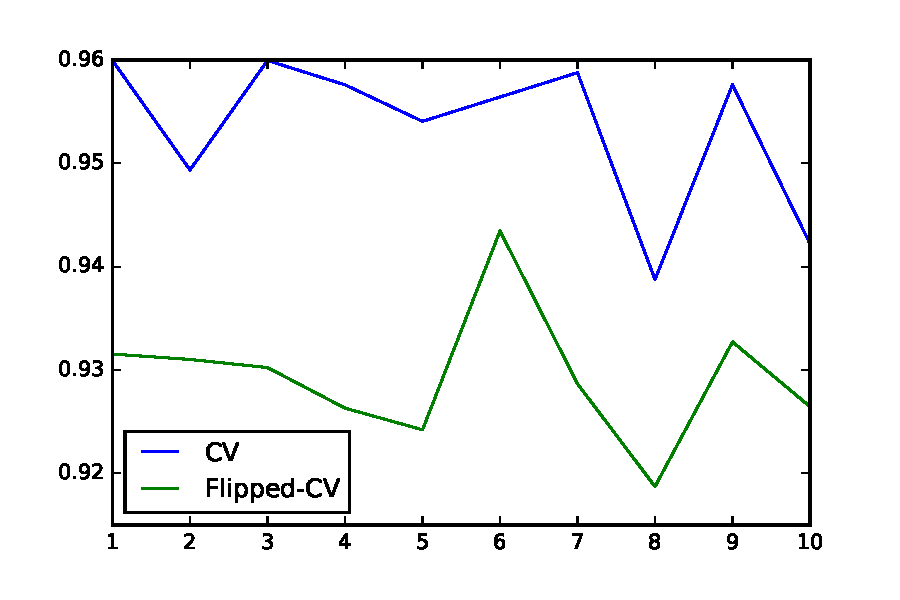
\includegraphics[width=0.75\linewidth]{studies/stylevar2017/accuracy.pdf}
	\caption{\label{stylevar2017:fig:cv}Accuracies for each fold over two complementary approaches: cross-validation (CV) and \textit{flipped} cross-validation (``flipped-CV"). \textit{Flipped} cross-validation takes 90\% of our dataset for training. The graph shows that both methods yield good results: in other words training on just 10\% of the dataset yields results that are just few points lower than normal cross-validation.}
\end{figure}

\begin{figure}[h]
	\centering 
	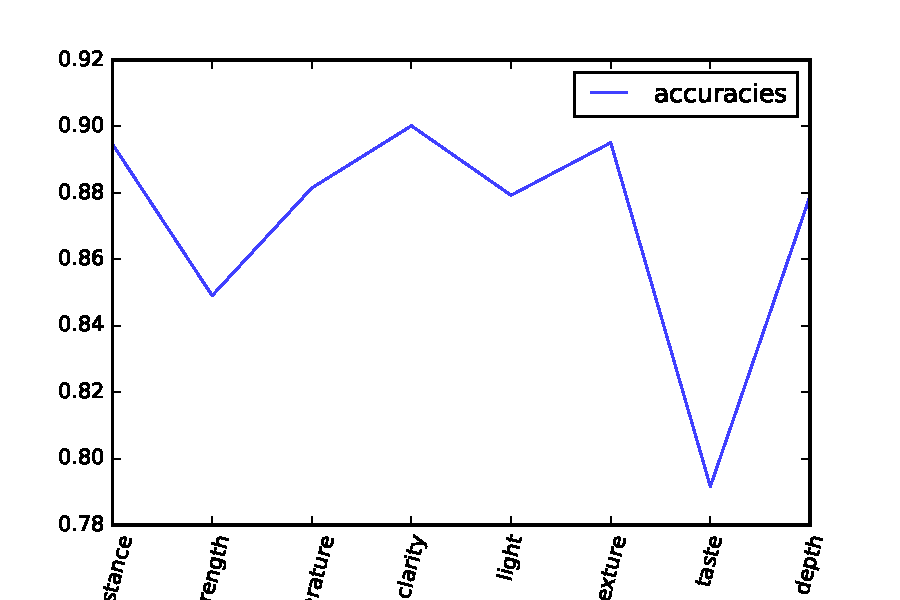
\includegraphics[width=0.75\linewidth]{studies/stylevar2017/adjs_acc.pdf}
	\caption{\label{stylevar2017:fig:adj}Accuracy training on different categories of adjectives. In this experiment, we train on just one category of the dataset and test on all the others. In general, training on just one category (e.g.\textit{temperature}) and testing on all other categories still yields high accuracy. While the power of generalization of our model is still unclear, we can see that it can detect similar semantic mechanisms even without any vocabulary overlap.  The category \textit{taste} is a partial exception: this category seems to be a relative ``outlier". }
\end{figure}


\begin{figure*}[h]
	\centering
	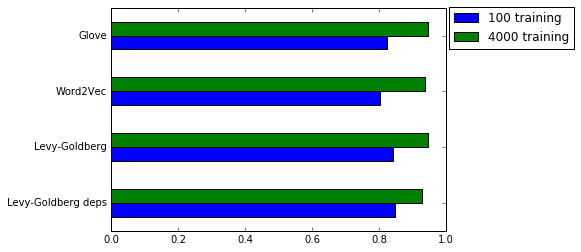
\includegraphics[width=0.85\linewidth]{studies/stylevar2017/embeddings.png}
	\caption{\label{stylevar2017:fig:emb} Accuracy on different kinds of embeddings, both training on 100 phrases and 4000 phrases.}
\end{figure*}

\begin{table}[t]
	\centering
	\begin{tabular}{|c c| c  c  c |}
	\hline
	Test & Train & Accuracy & Precision & Recall \\
	\hline
	6929 & 72   &  0.83 &   0.89 &  0.77 \\
	\hline
	5561 & 299  &  0.89 &   0.86 &  0.93 \\
	\hline
	4406 & 643  &  0.91 &   0.92 &  0.90 \\
	\hline
	3239 & 1203  &  0.90 &   0.91 &  0.88 \\
	\hline
	2253 & 1961  &  0.91 &   0.92 &  0.92 \\
	\hline
	1568 & 2763  &  0.89 &   0.90 &  0.90 \\
	\hline
	707  & 4291  &  0.91 &   0.94 &  0.91 \\
	\hline
	313  & 5494  &  0.93 &   0.92 &  0.95 \\
	\hline
	148  & 6282  &  0.93 &   0.94 &  0.92 \\
	\hline
	\end{tabular}
	\vspace{0.5em}
	\caption{\label{stylevar2017:tab:voc-split} This table shows consistent results in accuracy, precision and recall of the classifier trained with different split points of vocabulary instead of phrases. Splitting the vocabulary creates different sizes of training phrases and test phrases.}
\end{table}

\begin{table}[t]
	\centering
	\begin{tabular}{|c|p{5cm}|}
	\hline 
	\textbf{Top ten} & reluctance,
	 reprisal,
	 resignation,
	 response,
	 rivalry,
	 satisfaction,
	 storytelling,
	 supporter,
	 surveillance,
	 vigilance \\
	\hline 
	\textbf{Bottom ten} &
	saucepan,
	flour,
	skillet,
	chimney,
	jar,
	tub,
	fuselage,
	pellet,
	pouch,
	cupboard
	 \\
	\hline 
	\end{tabular}
	\vspace{0.5em}
	\caption{\label{stylevar2017:tab:polar} 10 most similar and  10 least similar terms with respect to the ``metaphoricity vector", concatenated using an all-zeros vector for the adjective. In practice, this is a way to explore which semantic dimensions are particularly useful to the classifier. A concrete/abstract polarity on the nouns was apparently derived}
\end{table}


\section{Discussion and future work}

In this paper we have presented an approach for detecting metaphoricity in AN pairs that out-performs the state of the art without using human annotated data or external resources beyond pre-trained word embeddings. We treasured the information captured by Word2Vec vectors through a fully connected neural network able to filter out the "noise" of the original semantic space. We have presented a series of alternative variations of this approach and evaluated its performance under several conditions - different word embeddings, different training data and different training sizes - showing that our model can generalize efficiently and obtain solid results over scarce training data.  We think that this is one of the central findings in this paper, since many semantic phenomena similar to metaphor (for example other figures of speech) are under-represented in current NLP resources and their study through supervised classifiers would require systems able to work on small datasets.  


The possibility of detecting metaphors and assigning a degree of ``metaphoricity" to a snippet of text is essential to automatic stylistic programs designed to go beyond ``shallow features" such as sentence length, functional word counting etc. While such metrics have already allowed powerful studies, the lack of tools to quantify more complex stylistic phenomena is evident \citep{hughes2012quantitative,gibbs2017metaphor}.  Naturally, this work is intended as a first step: the  ``metaphoricity" degree our system is learning would mirror the kinds of combination present in this specific dataset, which represents a very specific type of metaphor. 


It can be argued that we are not really learning the defining ambiguities of an adjective (e.g. the double meaning of ``bright") but that we are probably side-learning nouns' degree of abstraction. This would be in harmony with psycholinguistic findings, since detecting nouns' abstraction seems to be one of the main mechanisms we recur to, when we have to judge the metaphoricity of an expression \cite{cogni15} and is used as a main feature in traditional Machine Learning approaches to this problem. In other terms, our system seems to detect when the same adjective is used with different categories of words (abstract or concrete) and generalize over this distinction; a behavior that might not be too far from the way a human learns to distinguish different senses of a word. 


An issue that we would like to further test in the future is metaphoricity detection on different datasets, to explore the ability of generalization of our models. Researching on different datasets could also help us gaining a better insight about the model's learning.  

An obvious option is to test verb-adverb pairs (VA, e.g. \textit{think deeply}) using the same approach discussed in this paper. It would then be interesting to see whether having a common training set for both the AN and the VA pairs will allow the model to generalize for both cases or different training on two training sets, one for AN and one for VA, will be needed. Other cases to test include N-N compounds or proposition/sentence level pairs. 


Another way such an approach can be extended, is to investigate  whether reasoning tasks typically associated with different classes of adjectives can be performed. One task might be to distinguish adjectives that are intersective, subsective or none of the two. In the first case, from\textit{ A N x} one should infer that \textit{x} is both an \textit{A} and an \textit{N} (something that is a black table is both black and a table), in the second case one should infer that \textit{x} is \textit{N} only (for example someone who is a skillful surgeon is only a surgeon but we do not know if s/he is skillful in general), and in the third case neither of the two should be inferred. 
However, this task is not as simple as giving a training set with instances of AN pairs, to recognize  where novel instances of AN pairs belong to. 
Going beyond logical approaches by having the ability to recognize different uses of an adjective requires a richer notion of context which extends way beyond the AN-pairs. %


A further idea we want to pursue in the future is the development of more fine grained datasets, where metaphoricity is not represented as a binary feature but as a gradient property. This means that a classifier should have the ability to predict a degree of metaphoricity and thus allow more fine-grained distinctions to be captured. This is a theoretically interesting side and definitely something that has to be tested since not much literature is available (if at all) on gradient metaphoricity.  It seems to us that similar approaches, quantifying a text's metaphoricity and framing it as a supervised learning task, could help having a clear view on the influence of metaphor on style. 


\clearpage
\bibliographystyle{acl_natbib}
\bibliography{studies/stylevar2017/emnlp2016.bib}
